\chapter{Context analysis}

\section{Datasets}
\label{chapter:datasets}
In the realm of super-resolution algorithms, the choice of the dataset can significantly influence the algorithm's training and ultimately its performance. Three key datasets in this domain are the OpenImage Dataset, the WorldStrat Dataset, and the Sen2Venus Dataset. Upon contrasting these datasets, it becomes evident that there are several trade-offs to consider. These trade-offs, depending on the nature of the super-resolution tasks to be performed, could significantly influence the choice of the dataset. The OpenImage Dataset, for instance, excels with its $HR$ image pairs that reach up to 0.5 meters. However, its $LR$ pairs are synthetically generated and are geographically limited to the United States. Consequently, its global applicability may be limited, which could potentially constrain its utility in worldwide scenarios. The WorldStrat dataset, on the other hand, stands out with its diversity, offering a wide range of scenes and landscapes. This diverse sampling can enhance the generalization capabilities of SR algorithms. However, its approach of not filtering low-resolution revisits by their cloud coverage introduces an additional layer of complexity. Additionally, it is quite small in comparison to the size if the models. Lastly, the Sen2Venus Dataset is noted for its well-managed pre-processing that assures good correspondence between $LR$ and $HR$ images in the spectral domain. However, the $HR$ image has only double the spatial resolution of the $LR$ image and may lack the diversity found in the WorldStrat dataset. Below, we provide a more detailed explanation of each dataset.

\subsection{OpenImages}
OpenImages is a popular computer vision dataset that provides a large collection of labeled images for training and evaluating machine learning models. The dataset covers a wide range of visual concepts and objects, including people, cars, houses, trains, animals, etc.  It is widely used in tasks such as object detection, image classification, and visual relationship detection. For SR purposes, the amount and quality of the annotations are not of importance, but rather that it is an easily accessible and freely available dataset (CC-BY) containing over  millions images. The original authors of the latent-diffusion model used this dataset to train their checkpoints.

Since it is a computer vision dataset, it only contains RGB images of every-day scenes taken with standard digital cameras. Not only are therefore the objects depicted in the images completely unrelated to the remote sensing domain, their spectral characteristics are vastly different as well. In order to train 4 band models, a 4th band is artificially created from the image intensity and appended in the band dimension. The $LR$ image is created by interpolating the $HR$ version to the desired size of $128x128$ pixels.

The data in question is not directly connected to the research problem in terms of its spectral, spatial, or domain characteristics. However, the large volume of images proves valuable for training a freshly initialized model on fundamental image attributes and connections. Surprisingly, when applying super-resolution techniques to remote sensing imagery using autoencoders and denoising U-Nets trained on the OpenImages dataset, remarkably good results have been achieved. This demonstrates that the knowledge acquired through training on the OpenImages dataset can be transferred to the remote sensing domain and create a solid base for finetuning on more sophisticated datasets.

\begin{figure}[H] 
    \caption{\doublespacing \\ \textit{Example of an OpenImages LR and HR image pair.}} 
    \centering
    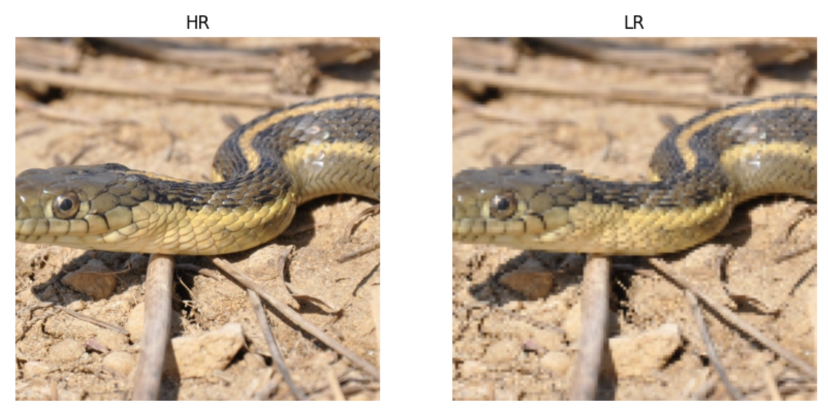
\includegraphics[width=1\linewidth]{images/openimages_example.png}
    \begin{justify}
        \textit{Note.} Example of an OpenImages LR and HR image pair.
    \end{justify}                    
    \label{fig:openimages_example}
\end{figure}

\subsection{Sentinel-2 Dataset}


\subsection{NAIP Dataset}
The National Agriculture Imagery Program (NAIP) acquires high-resolution aerial imagery of agricultural areas in the United States. It provides current and accurate imagery to support agricultural applications and decision-making. NAIP captures imagery at a spatial resolution of 0.6 meters, allowing for detailed analysis of agricultural activities. Using specialized aerial platforms with multispectral sensors, NAIP collects data in various spectral bands, including red, green, blue, and near-infrared. The NAIP dataset covers diverse agricultural regions and is regularly updated. It is freely available to the public, facilitating its use in agricultural research, precision farming, land management, and related applications. A comparison between Sentinel-2 and NAIP is shown in Figure \ref{fig:naip_comparison}.

\begin{figure}[H] 
    \caption{\doublespacing \\ \textit{Comparison between Sentinel-2 and NAIP near Rapid City, South Dakota.}} 
    \centering
    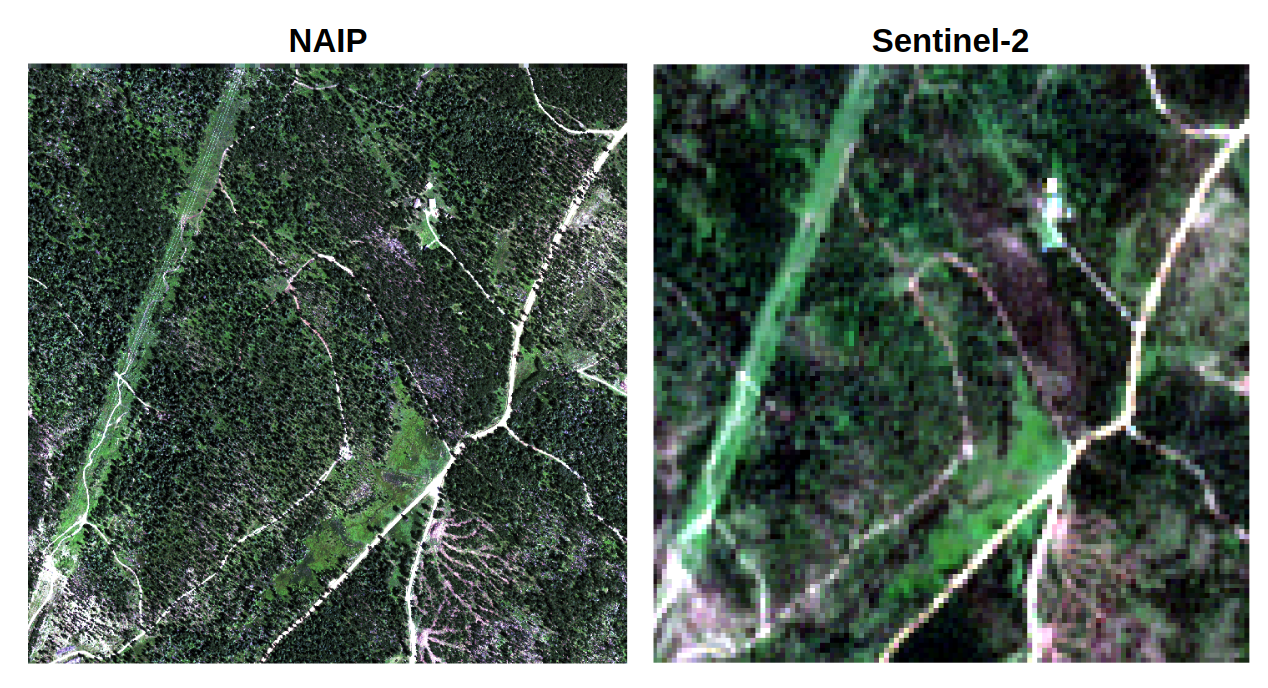
\includegraphics[width=1\linewidth]{images/csaybar_fig02.png}
    \begin{justify}
        \textit{Note.} Comparison between Sentinel-2 and NAIP near Rapid City, South Dakota. The Sentinel-2 image (rigth) has a spatial resolution of 10 meters, while the NAIP image (left) has a spatial resolution of 0.6 meters.
    \end{justify}                    
    \label{fig:naip_comparison}
\end{figure}


\subsection{OpenSR dataset}
The OpenSR dataset is an extensive dataset designed to facilitate the development of standard and reference single-image super-resolution algorithms for Sentinel-2 imagery. The high-resolution (HR) images in this dataset are sourced from the National Agriculture Imagery Program (NAIP), which provides aerial imagery covering the entire contiguous United States.

NAIP collects data across various spectral bands, including red, green, blue, and near-infrared, at a resolution of 0.6 m/pixel.

\subsection{WorldStrat Dataset}
The World Stratified Dataset, also known as WorldStrat, is a curated and diverse dataset. Its primary purpose is to aid in the development of multi-frame super-resolution algorithms specifically designed for Sentinel-2 imagery. A key feature of this dataset is the inclusion of high-resolution (HR) imagery from the SPOT 6/7 satellites. The SPOT imagery encompasses five distinct spectral bands. The panchromatic (PAN) band is at 1.5 m/pixel and the remaining bands, include Red, Green, Blue, and Near Infrared (RGBNIR) at 6 m/pixel.

The dataset covers approximately 10000 square kilometers and includes 3504 distinct areas of interest \ref{fig:worldstrat}, curated for the highest diversity of possible uses. The image acquisition budget for the dataset is divided into three parts:

\begin{itemize}
    \item \textbf{Settlement/Urban:} This part covers 3,647.5 square kilometers with 1,459 high-resolution images. The images are stratified sampling based on urban density (SMOD).
    \item \textbf{Non-Settlement}: This part covers 2,370 square kilometers with 948 high-resolution images. The images are stratified sampling based on land use (IPCC).
    \item \textbf{Underrepresented}: This part covers 3802.5 square kilometers with 1521 high-resolution images. The sources for these images include UNHCR, Amnesty, and ASMSpotter.
\end{itemize}

\begin{figure}[H] 
    \caption{\doublespacing \\ \textit{Summarizing the construction and classes of the WorldStrat dataset.}} 
    \centering
    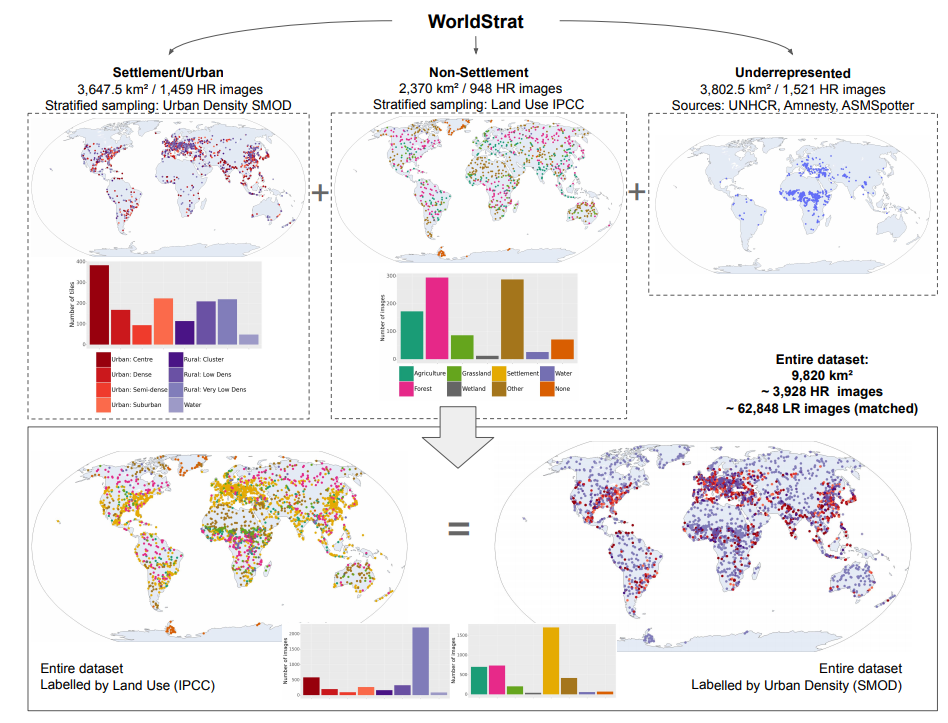
\includegraphics[width=1\linewidth]{images/csaybar_fig07.png}
    \begin{justify}
        \textit{Note.} Summarizing the construction and classes of the WorldStrat dataset. Obtained from \textcite{cornebise2022open}
    \end{justify}                    
    \label{fig:worldstrat}
\end{figure}


\subsection{Sen2Venus Dataset}

SEN2VENμS is a large dataset specifically designed to improve the spatial resolution of eight Sentinel-2 bands to 5 meters. It consists of cloud-free surface reflectance patches captured by Sentinel-2 L2A at 10 meters and 20 meters, along with corresponding reference patches acquired by the VENμS satellite at 5-meter resolution on the same day. The dataset covers 29 different locations worldwide, encompassing a total of 132,955 patches, each with a size of 256 × 256 pixels 

SEN2VENµS is a large dataset specifically designed to improve the spatial resolution of eight Sentinel-2 bands to 5 meters. It consists of cloud-free surface reflectance patches captured by Sentinel-2 L2A at 10 meters and 20 meters, along with corresponding reference patches acquired by the VENµS satellite at 5-meter resolution on the same day. The dataset covers 29 different locations worldwide, encompassing a total of 132,955 patches, each with a size of 256 × 256 pixels (Figure \ref{fig:sen2venus}).

\begin{figure}[H] 
    \caption{\doublespacing \\ \textit{Map of Sentinel-2 coverage on Theia (orange), available VENμS sites (green).}} 
    \centering
    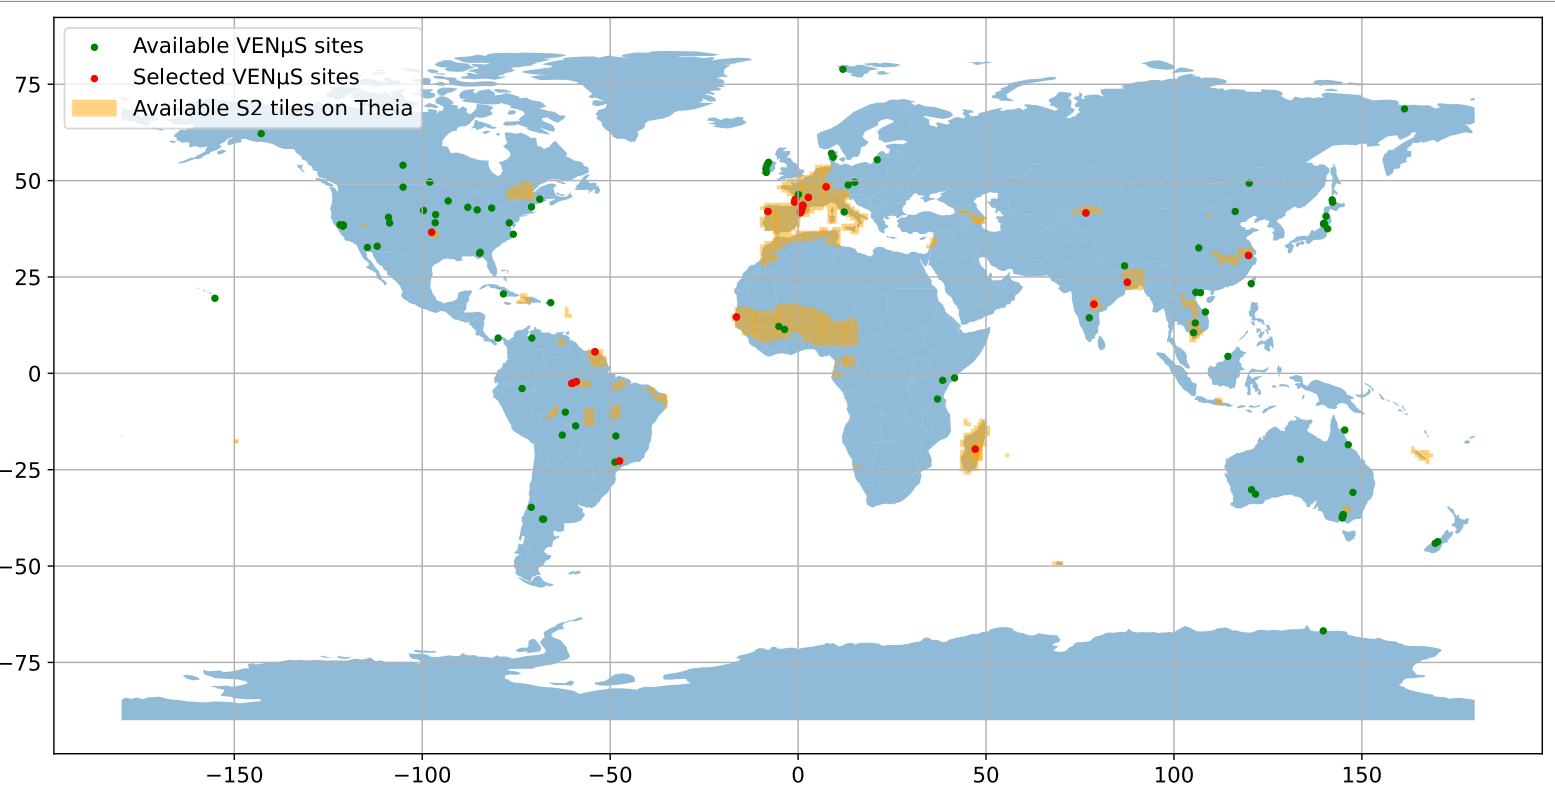
\includegraphics[width=1\linewidth]{images/csaybar_fig06.png}
    \begin{justify}
        \textit{Note.} Map of Sentinel-2 coverage on Theia (orange), available VENμS sites (green) and 29 selected sites (red) for the dataset. Obtained from \textcite{michel2022sen2venmus}
    \end{justify}                    
    \label{fig:sen2venus}
\end{figure}


\subsection{Degraded Sentinel-2 Dataset}

The datasets introduced above all have certain qualities and drawbacks. One of the factors to balance is dataset size compared to the quality and suitability of the data. On one end of the spectrum, WorldStrat is of very high quality and closely connected to the type of SR we want to perform, while on the other end the OpenImages dataset is huge while having no connection to remote sensing imagery. In order to have images in the spectral domain of Sentinel-2 and from the remote sensing domain, a large amount of Sentinel-2 RGB-NIR imagery has been sampled all over the world (Figure \ref{fig:sampling_sites}).

The images of course have the standard Sentinel-2 resolution of 10 meters, which is used as the $HR$ version. The $LR$ version of the image pair is created by applying a degradation kernel to the $HR$ image, producing a pair of $LR$-$HR$ RGB-NIR images that have 40 and 10m spatial resolution respectively, for a SR factor of 4. Over 250,000 image pairs are created this way, providing a dataset that has no problems with a spectral, temporal or geometrical mismatch and is already in the domain of Sentinel-2. The only drawback is that the frequency of information is changed since the scale of objects on the ground is vastly different. Still, this dataset is very useful in training the networks either from scratch or for a rougher finetuning after being trained on natural image datasets. After that, the NAIP and worldstrat datasets can provide the final touch.

\begin{figure}[H] 
    \caption{\doublespacing \\ \textit{Sampling areas (gray) and locations (red) of cloud-free Sentinel-2 images.}} 
    \centering
    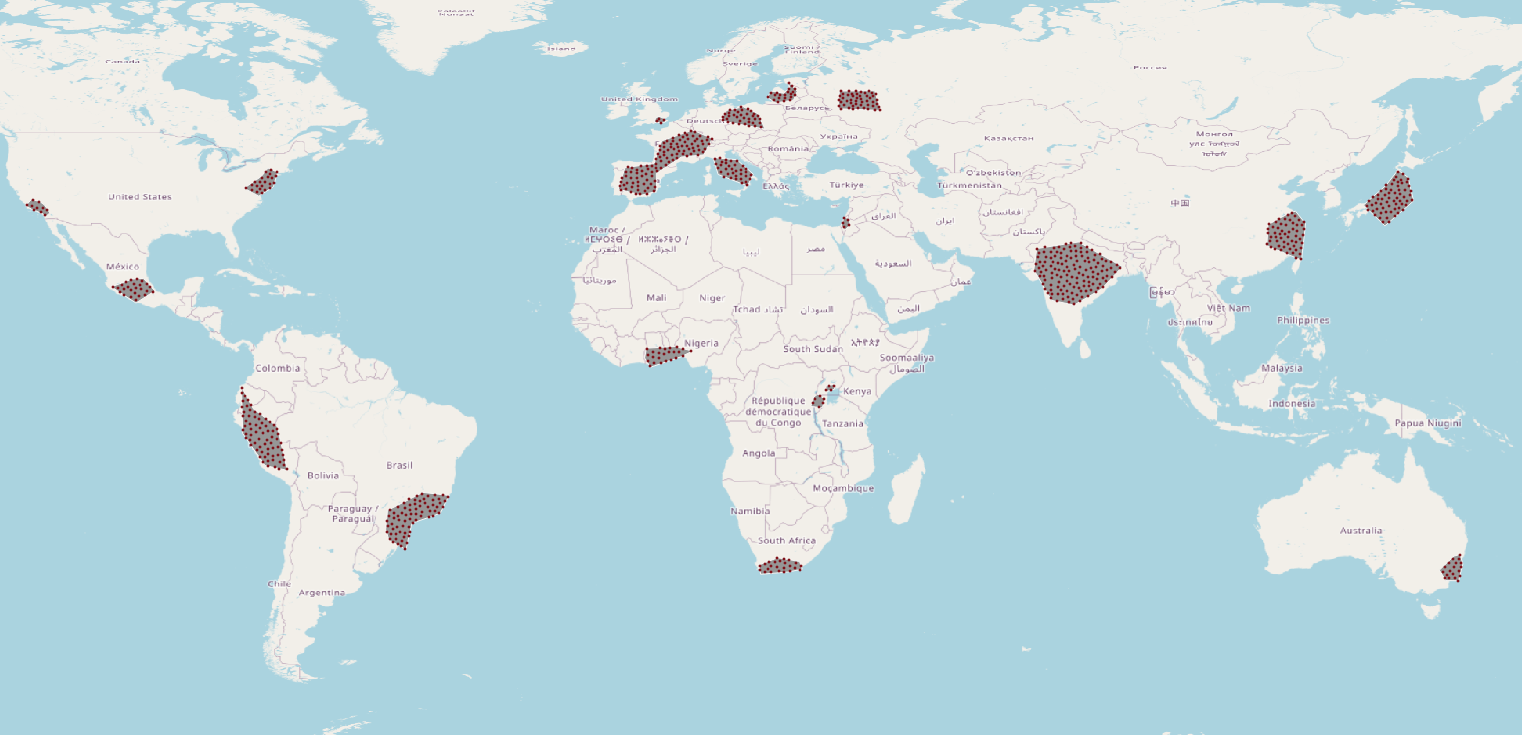
\includegraphics[width=1\linewidth]{images/sampling_locations.png}
    \begin{justify}
        \textit{Note.} Sampling areas (gray) and locations (red) of cloud-free Sentinel-2 images.
    \end{justify}                    
    \label{fig:sampling_sites}
\end{figure}

\begin{figure}[H] 
    \caption{\doublespacing \\ \textit{Example of the degraded Sentinel-2 dataset.}} 
    \centering
    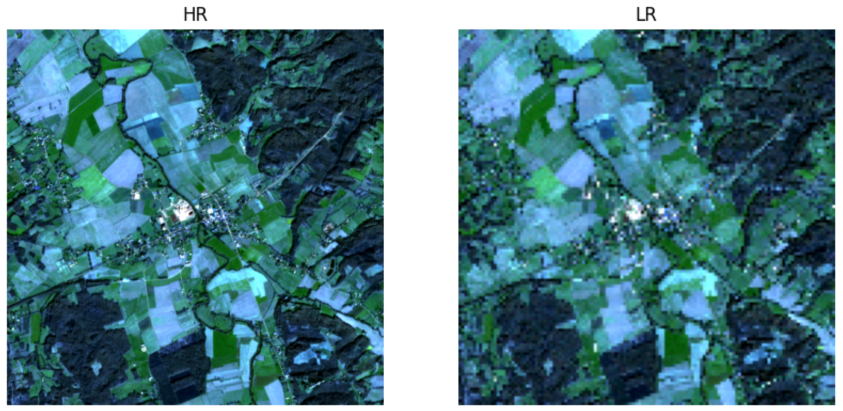
\includegraphics[width=1\linewidth]{images/sen2_degr.png}
    \begin{justify}
        \textit{Note.} Example of the degraded Sentinel-2 dataset (HR: 10m, LR: 40m). While the spectral properties as unmistakable Sentinel-2-like, the spatial information frequency is clearly different from 2.5m-10m datasets.
    \end{justify}                    
    \label{fig:sen2_degraded}
\end{figure}


\section{Data Harmonization}

\subsection{Effective spatial resolution and PSF}

Understanding the relationship between effective spatial resolution and the Point Spread Function (PSF) is essential for accurate interpretation of super-resolution models. In our study, the term effective spatial resolution is employed to denote the spatial resolution as gauged by the ground sampling distance, rather than simply characterizing it by the pixel size. The concept of ground sampling distance (GSD) refers to the system's capability to delineate small objects within an image. The GSD is influenced by various factors, including sensor design, viewing angle, and image pre-processing techniques. These factors can be effectively modeled using single or multiple PSFs (Figure \ref{fig:psf}).


\begin{figure}[H] 
    \caption{\doublespacing \\ \textit{A graphical depiction illustrating the Point Spread Function (PSF) of an optical imaging system.}} 
    \centering
    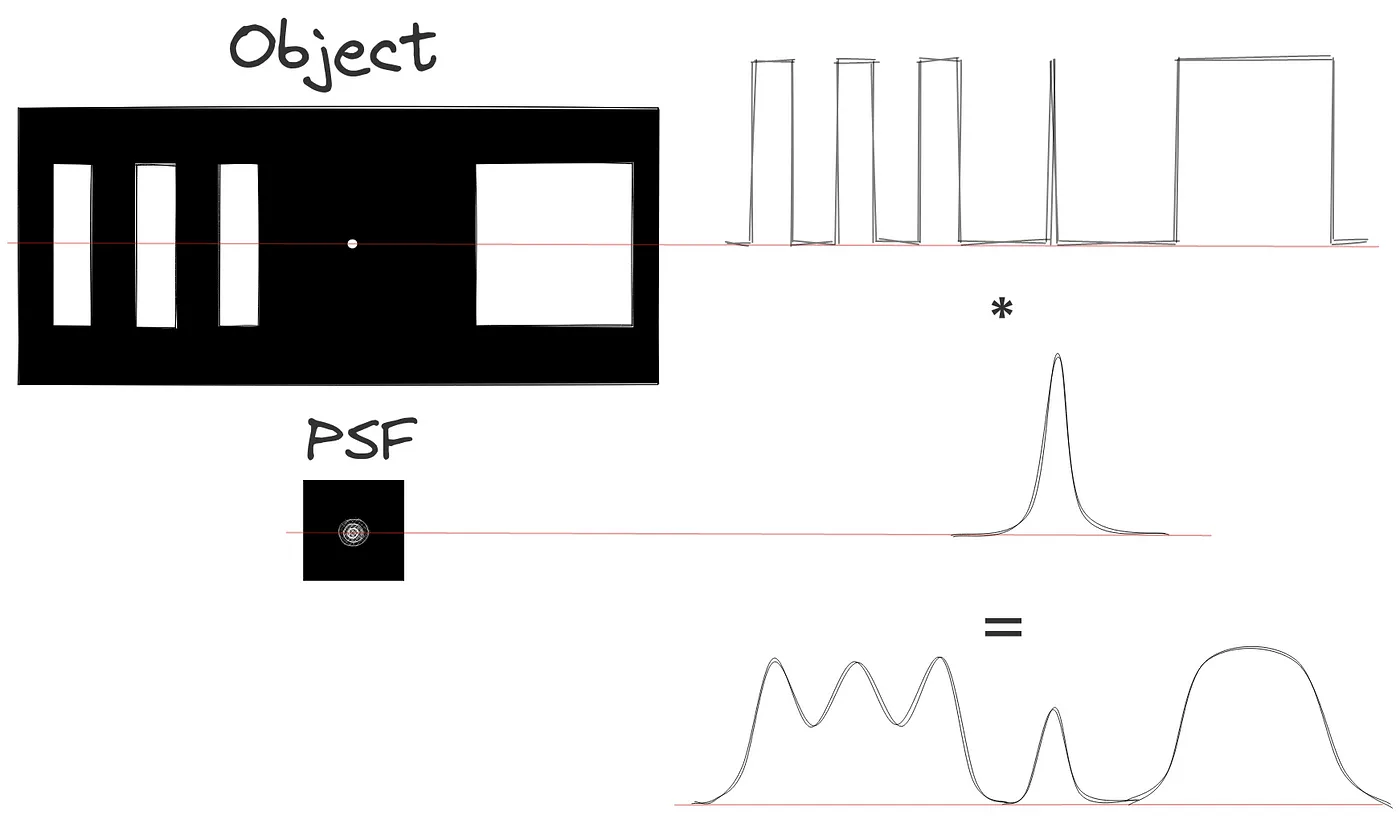
\includegraphics[width=1\linewidth]{images/csaybar_new_fig01.png}
    \begin{justify}
        \textit{Note.} A graphical depiction illustrating the Point Spread Function (PSF) of an optical imaging system. The extent of the spread directly impacts the spatial resolution, meaning that when it is larger, the ability to distinguish individual objects decreases.
    \end{justify}                    
    \label{fig:psf}
\end{figure}


The PSF characterizes the response of an imaging system to a point source or a single pixel. It describes how the energy from an object spreads out in the image, affecting image sharpness, resolution, and spatial accuracy. Through the modeling of the PSF attributes, it is possible to emulate the functionalities of low-resolution ($LR$) remote sensing systems using high-resolution ($HR$) counterparts.

\subsection{Spatial Co-registration}

In the realm of super-resolution, spatial co-registration serves as an essential preprocessing measure to mitigate disparities between high-resolution ($HR$) and low-resolution ($LR$) sensors. In practical scenarios, even marginal misalignments can considerably influence the precision of the resultant metrics. Consequently, guaranteeing meticulous spatial co-registration becomes indispensable for deriving trustworthy and insightful super-resolution metrics.

Spatial co-registration algorithms generally encompass three primary stages. The first stage is keypoint detection, which seeks to identify prominent points within an image. The next stage involves the detection of matching points between the $HR$ and $LR$ images. Lastly, the misalignment errors are calculated through a polynomial model fitted to these matching points. Over recent years, a plethora of algorithms for automated image alignment have been presented. For instance, the SEN2VENμS dataset utilized the SIFT matching algorithm \autocite{michel2022sen2venmus}, while MuRA-T compare the alignment outcomes of Fast+VGG and SuperPoint+SuperGlue algorithms \autocite{deshmukh2023aligned}.

\begin{figure}[H]
    \caption{\doublespacing \\ \textit{Matching points obtained by applying the SuperPoint + SuperGlue algorithm to a pair of images.}} 
    \centering
    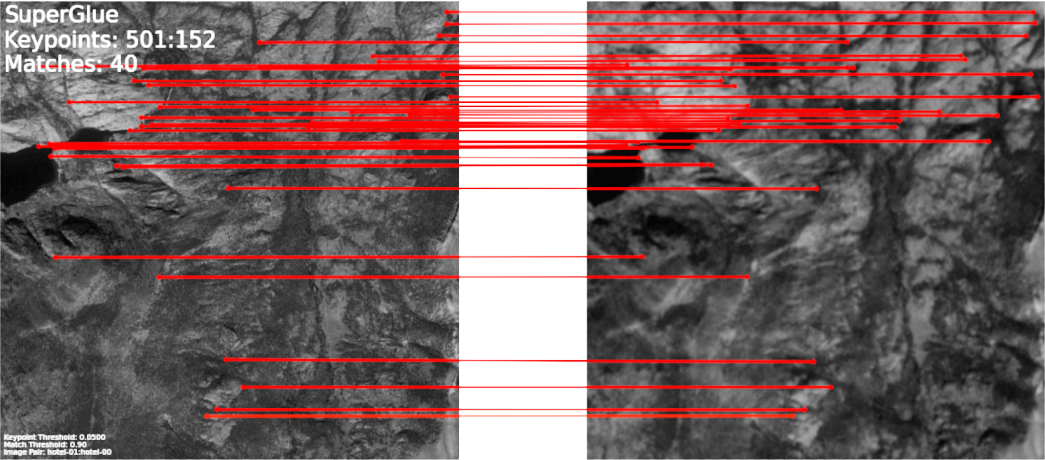
\includegraphics[width=1\linewidth]{images/csaybar_fig01.png}
    \begin{justify}
        \textit{Note.} Matching points obtained by applying the SuperPoint + SuperGlue algorithm to a pair of images, where the low-resolution (LR) image is from Sentinel-2 and the high-resolution (HR) image is from NAIP.
    \end{justify}                    
    \label{fig:coregistration}
\end{figure}

\subsection{Cross-instrument calibration and harmonization}
Even when two remote sensing sensors acquire data on the same day, significant variations in their values may still exist. These variations can be attributed to several factors, which include:


\begin{itemize}
    \item \textbf{Sensor characteristics}: Each sensor has its own unique spectral response function, which can result in variations in the reflectance values, even when the atmospheric conditions and viewing angle are the same.

    \item \textbf{Atmospheric conditions}: The atmosphere can undergo significant changes within a few minutes or seconds. These variations can impact the quality and accuracy of the data captured by remote sensing sensors. Atmospheric scattering, for example, can introduce variations in the sensor signals, leading to differences in reflectance values.

    \item \textbf{Viewing geometry}: The difference between the angle at which the sensors observe the Earth's surface, can also lead to variations in the reflectance values.

    \item \textbf{Calibration and preprocessing}: Each sensor goes through its own calibration process to convert the raw sensor measurements into meaningful reflectance values. These variations need to be carefully accounted for and addressed during $LR$-$HR$ comparison.
    
\end{itemize}

To minimize potential variations in reflectance between $LR$-$HR$ pairs, an additional component is proposed to enhance the classical degradation model.

\begin{equation}
    I_{LR} = \gamma[\delta(I_{HR}, \eta)] + \epsilon
\end{equation}

Where $I_{LR}$ is the $LR$ image, $I_{HR}$ is the $HR$ image, $\eta$ is a parameter from the degradation model $\delta$, $\epsilon$ represent the noise, and the $\gamma$ the harmonization model.